\documentclass[11pt]{article}
\usepackage{setspace}
\setstretch{1}
\usepackage{amsmath,amssymb, amsthm}
\usepackage{graphicx}
\usepackage{bm}
\usepackage[hang, flushmargin]{footmisc}
\usepackage[colorlinks=true]{hyperref}
\usepackage[nameinlink]{cleveref}
\usepackage{footnotebackref}
\usepackage{url}
\usepackage{listings}
\usepackage[most]{tcolorbox}
\usepackage{inconsolata}
\usepackage[papersize={8.5in,11in}, margin=1in]{geometry}
\usepackage{float}
\usepackage{caption}
\usepackage{esint}
\usepackage{url}
\usepackage{enumitem}
\usepackage{subfig}
\usepackage{wasysym}
\newcommand{\ilc}{\texttt}
\usepackage{etoolbox}
\usepackage{algorithm}
\usepackage{changepage}
% \usepackage{algorithmic}
\usepackage[noend]{algpseudocode}
\usepackage{tikz}
\usetikzlibrary{matrix,positioning,arrows.meta,arrows}
\patchcmd{\thebibliography}{\section*{\refname}}{}{}{}
% \PassOptionsToPackage{hyphens}{url}\usepackage{hyperref}

\providecommand{\myceil}[1]{\left \lceil #1 \right \rceil }
\providecommand{\myfloor}[1]{\left \lfloor #1 \right \rfloor }


\begin{document}



\title{\textbf{CSDS 455: Homework 18}}

\author{Shaochen (Henry) ZHONG, \ilc{sxz517}}
\date{Due and submitted on 10/26/2020 \\ Fall 2020, Dr. Connamacher}
\maketitle

\textit{I have consulted Yige Sun and \url{https://www.researchgate.net/publication/229747655} for the following problems.}

\section*{Problem 1}

If the contracted edge $e$ is a part of a chordal (3-edge) circle in $G$, then after the contraction every chordal circle including this $e$ will be ``collapsed'' to a line, and such collapse will not creating any non-chordal structure, thus the graph is still chordal. If the contracted edge $e$ is not part of a chordal circle, then a contraction of $e$ won't affect the chordal property of the graph.

Since the graph is still chordal regardless which edge $e$ is contracted, the statement is therefore proven.

\section*{Problem 2}
Known that every planar graph can be drawn in a plane graph format, we convert our planar $G$ to plane $G$ -- we may say that if a minor of plane $G$ is still plane, it must be planar.\newline

It is trivial that edge or vertex deletion will not make a plane graph no longer plane. For edge contraction, say we are contraction edge of $xy$ into vertex $x'$. Due to the plane graph property, edge coming out of $x$ or $y$ are not crossing any other edges, and therefore so do edges comming out of $x'$ after the contraction.

Since we have showed a plane graph $G$ will still be plane graph after all three possible minor-manuvers, a minor of $G$ must be a planar graph.

\section*{Problem 3}

Base on the given instruction, of $\chi(G') \geq k$, then the proof is trivial as we know that such $G'$ will have a $K_k$ minor, and therefore by removing a vertex out of this $K_k$ minor, ad have a $K_{k-1}$ minor.

If $\chi(G') \not \geq k$, in other another word  $\chi(G') = k-1$, we now add a vertex $v$ to $G'$ where $v$ is connected to all vertices of $G'$. Now there must be $\chi(G' + v) = k$ and therefore has a $K_k$ minor, we then proceed to solve it by cases:

\begin{itemize}
    \item If $v$ is part of the $K_k$ minor of $G' + v$. Then this suggests there must be a $K-1$ vertices of the $K_k$ minor in $G'$, where any two of them a connected. So we can identify these $K-1$ vertices inside $G'$ and deletion/contraction according to achieve a $K_{k-1}$ minor out of $G'$.
    \item If $v$ is not in the $K_k$ minor of $G' + v$ due to deletion or simply not included in the $K_k$ minor, that means $G'$ already has a $K_k$ in itself and we can make a $K_{k-1}$ minor out of $K_k$ minor by removing one vertex (this is in fact not a case of $\chi(G' + v) = k$).
    \item If $v$ is not in the $K_k$ minor of $G' + v$ due to edge contraction. Say $v$ is contracted with vertex $u$ to make $v'$ and this $v'$ is in the $K_k$ minor of $G' + v$. Then we can simply remove this $v'$ to make a $K_{k-1}$ minor.
\end{itemize}

Since we may obtain a $K_{k-1}$ minor out of $G'$ in every case, the statement is therefore proven.

\section*{Problem 4}


The base case will be $|V(G)|=1$, which does not contain $K_4$ minor and is certainly 3-colorable. We assume that this is true for $|V(G)| \leq k-1$.\newline

For any graph with $|V(G)| = k$ (we only consider connected non-tree graph, as every tree is 2-colorable), we pick an edge $e$ between verticies $u, v$. Denotes the minimum vertex cut between $u, v$ to be $x$, we know this $x$ must be a independent set (i.e. no verteices within $x$ are internally connected), as otherwise (assuming $x_1, x_2$ are connected) we have path of $uv, ux_1, u_x2, v_1, v_x2, x_1 x_2$ which can produce a $K_4$ minor.


\begin{figure}[H]
    \centering
    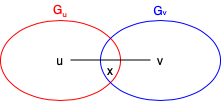
\includegraphics[width=0.4\linewidth]{{fig/fig_p4_1.png}}
\end{figure}

After the vertex cut between $u, v$, we now denote the partition including $u$ plus $x$ to be $G_u$, and likewise the parition including $v$ plus $v$ to be $G_v$. Namely, we have $G_u \cap G_v = x$ and $G_u \cup G_v = G - e$. Now we do edge contraction to $G_u$ so that every verteices of $G_u$ is contracted to one vertex $u'$, we denote the graph $G$ with contracted $G_u$ as $G'_u$; and likewise we denote the graph $G$ with contracted $G_v$ to one vertex $v'$ as $G'_v$.\newline

As $|V(G'_u), |V(G'_v)| < k$ and neither of them has a $K_4$ minor, by the induction assumption they are 3-colorable. This means, the $x$ portion of $G'_u$ can be colored as $c_1$, and the leftover $G'_u - x$ can be colored as $c_1, c_2, c_3$; similarily,  $x$ portion of $G'_v$ can be colored as $c_1$, and the leftover $G'_v - x$ can be colored as $c_1, c_2, c_3$. Note the

Then for $G$, we may color the $x$ portion of it as $c_1$, then we color vertices in $G_u - x$ exactly as their corresponding vertices in $G'_v - x$; similarily, we color vertices in $G_v - x$ exactly as their corresponding vertices in $G'_u - x$. This will give us a 3-color of $G-e$ as $G_u - x$ are not connected to $G_v - x$, so as long as each of them are 3-colorable and $x$ using one of the three colors, we have a 3-colored $G-e$.

Note it is possible that we may have $u, v$ colored as the same color. We know this color must be $c_2$ or $c_3$, as in $G'_u$ (W.L.O.G.) $v$ is connected to $u'$ (which includes all verticies in $x$), so $v$ must be using a different color to $x$. So if $u, v$ happen to be using the same color, say $c_2$, we may simply shift swap $c_2$-colored vertices to $c_3$ in $G_v - x$. With $u, v$ using different colors, we may add the $e$ back and have a 3-colored $G$.\newline

Since we haved showed that for $G$ with $|V(G)| = 1, k-1, k$ having no $K_4$ minor, such $G$ is 3-colorable, we may say that every $G$ that does not contain a $K_4$ minor is three colorable.



% W.L.O.G., we can make $u$ to be colored as $c_2$ and $v$ to be colored as $c_3$, where thezx






\end{document}